\documentclass[]{article}   	% use "amsart" instead of "article" for AMSLaTeX format
\usepackage[utf8]{inputenc}
\usepackage{graphicx}
\graphicspath{{./Pictures/}}

\title{Android Lego Rovers\\User Manual}		
\date{}			

\begin{document}


\maketitle
\renewcommand\abstractname{}
\abstract{This is the user manual for the lego rovers android project, in this manual we have used a samsung galaxy tab 3 with android kitkat 4.4 for the examples in the manual. This app will work on any android device with 4.4 (KitKat) or higher, though the procedure to connect will be the same the look of the menus may be different.}

\section{Prerequisites}
\par{To use this manual you will need the following items:
\begin{enumerate}
	\item One EV3 robot in dinosaur setup.
	\item One android KitKat (4.4) device with Bluetooth and the lego rovers app
\end{enumerate} 
}

\section{Connecting}
\par{To connect the android device and the EV3 robot with bluetooth is a two step process. First getting the android device to pair the EV3 robot over Bluetooth and then connecting the Lego Rovers app to the EV3 robot.}

\par{To ensure that the connection does take place the WiFi and mobile internet must be switched off.}

\clearpage
\subsection{Bluetooth Pairing}
\par{The first step is to get the android tablet to pair with the EV3 robot. To achieve this :
\begin{enumerate}
	\item Turn on the EV3 robot by pressing the dark grey button in the middle\\
		\begin{center}
			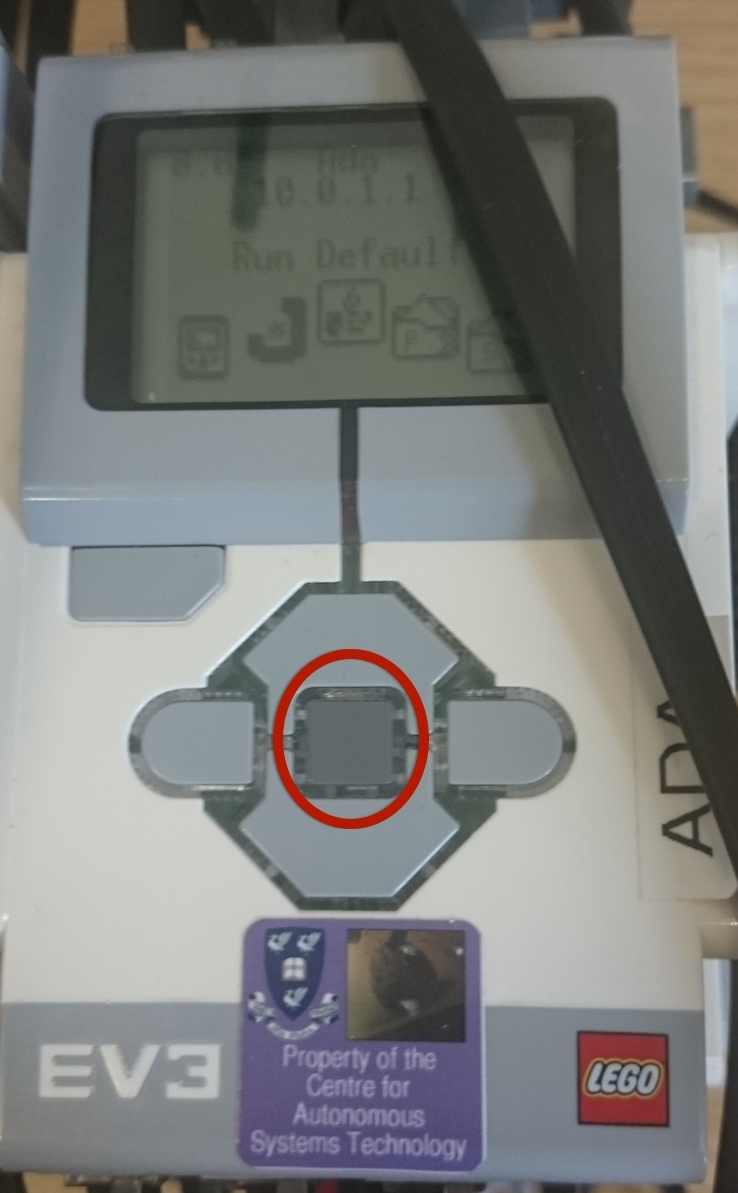
\includegraphics[scale=0.2]{graybtn.JPG}
		\end{center}		
	\item Wait for the EV3 to finish starting up, it will make a beep when it is ready. (This will take a while)
	\item Go into the settings app on your device\\
		\begin{center}
			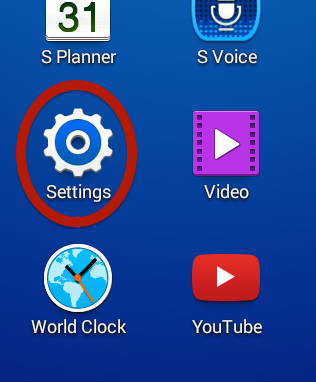
\includegraphics[scale=0.4]{settingapp.png}
		\end{center}			
	\item Turn on bluetooth	\\
		\begin{center}
			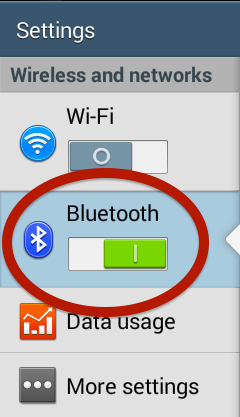
\includegraphics[scale=0.45]{btswitch.png}
		\end{center}			
	\item Touch the name of the robot when it appears.\\
		\begin{center}
			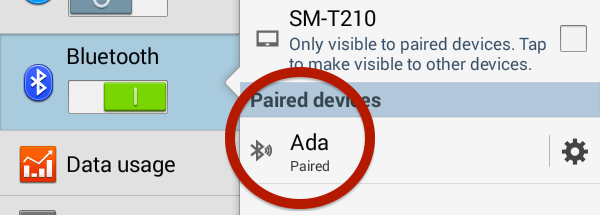
\includegraphics[scale=0.4]{btada.png}
		\end{center}			
	\item Touch the gear icon next to the robot name\\
		\begin{center}
			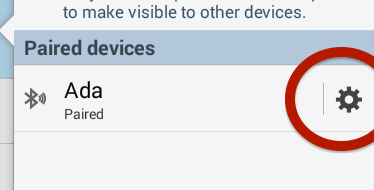
\includegraphics[scale=0.4]{btset.png}
		\end{center}		
\clearpage	
	\item Touch the box so that the internet enabled box is ticked\\
		\begin{center}
			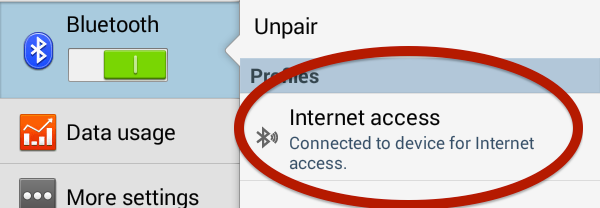
\includegraphics[scale=0.4]{btinternet.png}
		\end{center}		
	\item The pairing is now complete
	\item Make sure mobile data and WiFi is switched off
\end{enumerate}
\par{The next step is to connect the Lego Rovers app with the EV3 robot.}

\subsection{Connecting}
\par{After you have paired the device and the EV3 robot, you will need to connect the app to the EV3 robot to do this:
\begin{enumerate}
	\item Start the Lego Rovers app\\
		\begin{center}
			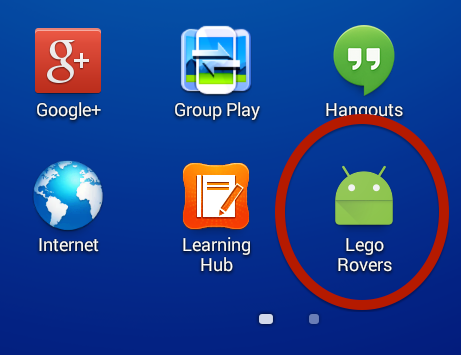
\includegraphics[scale=0.4]{apps.png}
		\end{center}		
\clearpage
	\item Go to settings with the Lego Rovers app\\
		\begin{center}
			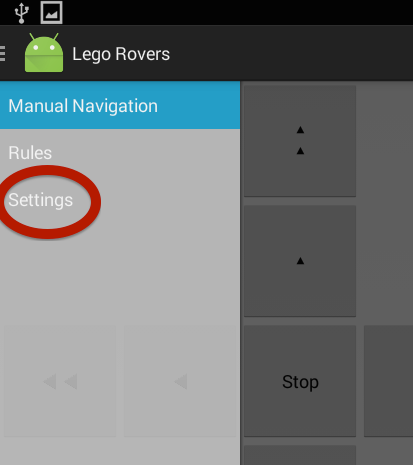
\includegraphics[scale=0.4]{navset.png}
		\end{center}		
	\item Press the connect button\\
		\begin{center}
			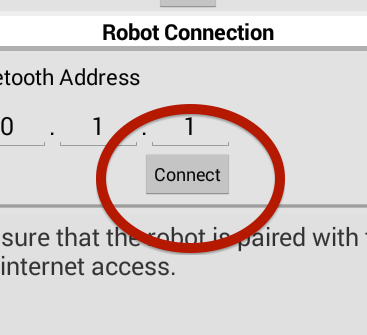
\includegraphics[scale=0.5]{connect.png}
		\end{center}		
	\item Wait for the connected message to appear beneath the button. 
\end{enumerate}

\par{The robot is now connected and ready to use.}
}



\section{App Usage}
\subsection{Navigating Screens}
\par{To select a screen to use first touch the menu item on the top left of the screen. A list of pages will appear, touch the page name to go to that page	}
\subsection{Manual Control}
\par{
\begin{center}
	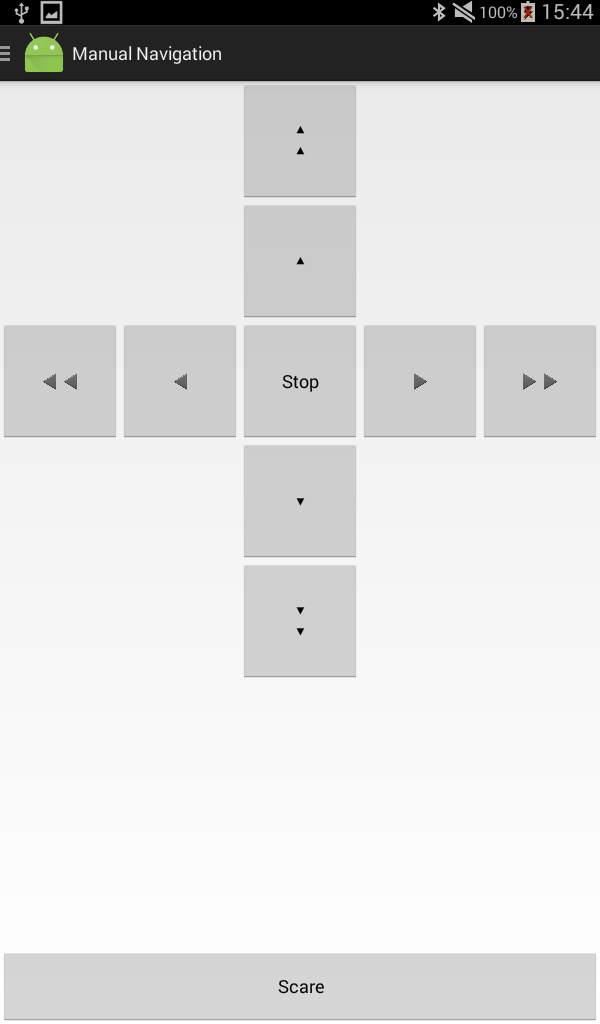
\includegraphics[scale=0.3]{navpane.png}
\end{center}			
}
\par{This screen has a number of buttons that can be pressed to control the robot, when connected the buttons do the following: 
\begin{description}
	\item[Double Up Arrow] Make the robot move forward until stop is pressed
	\item[Up Arrow] Makes the robot move forward a short distance
	\item[Stop] Stops the robot moving
	\item[Down Arrow] Makes the robot go backwards a short distance
	\item[Double Down Arrow] Makes the robot go backwards until the stop is pressed
	\item[Double Left Arrow] Makes the robot turn left until stop is pressed
	\item[Left Arrow] Makes the robot turn left, about 90 degrees
	\item[Right Arrow] Makes the robot turn right, about 90 degrees
	\item[Double Right Arrow] Makes the robot turn right until stop is pressed
	\item[Scare] Makes the ``Jaws" of the robot open and close twice
\end{description}
}

\subsection{Rules}
\par{
\begin{center}
	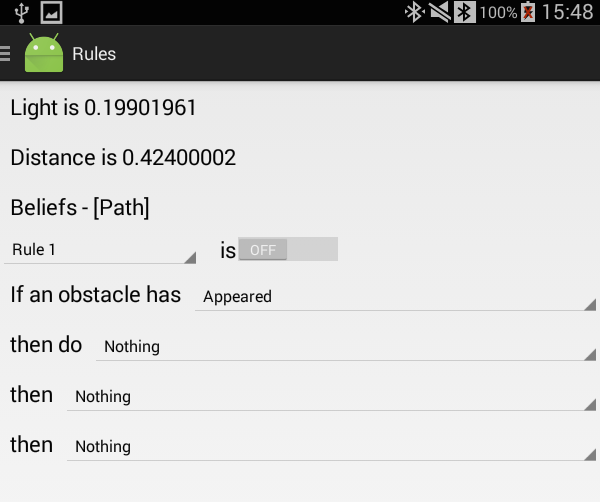
\includegraphics[scale=0.45]{rules.png}
\end{center}			
}
\par{The rules section allows you to create rules that the robot will do, when either faced with an object or an object has disappeared. This is split into two sections with the top being the current values of the sensors and the bottom being where you can create and edit the rules of the robot.}
\par{The top section consists of the following:
\begin{description}
\item[Light]This is the light sensor values, which returns the numerical value of the colour
\item[Distance]This is the distance an object is from the front of the robot.
\item[Beliefs]This is a list of what the robot believes to be true. Water being that the light sensor is picking up a blue colour, Path being that the light sensor is picking up a black colour and Obstacle being that an object is close to the front of the robot.
\end{description}
}

\par{The second section is for creating rules which the robot will do when either faced with an object or when the object has been moved out of the way of the robot. You can select a rule to change from the dropdown menu. The options for the rules include:
\begin{description}
	\item[On/Off Switch] This turns the rule on or off for the robot
	\item[Obstacle Choice] This dropdown menu lets you choose when the robot should react, either when an object has appeared or disappeared
	\item[Choice of Actions] There are a further three dropdown menus which allow you to choose what the robot should do in the event that the obstacle has appeared/disappeared
\end{description}
}

\subsection{Settings}
\par{
\begin{center}
	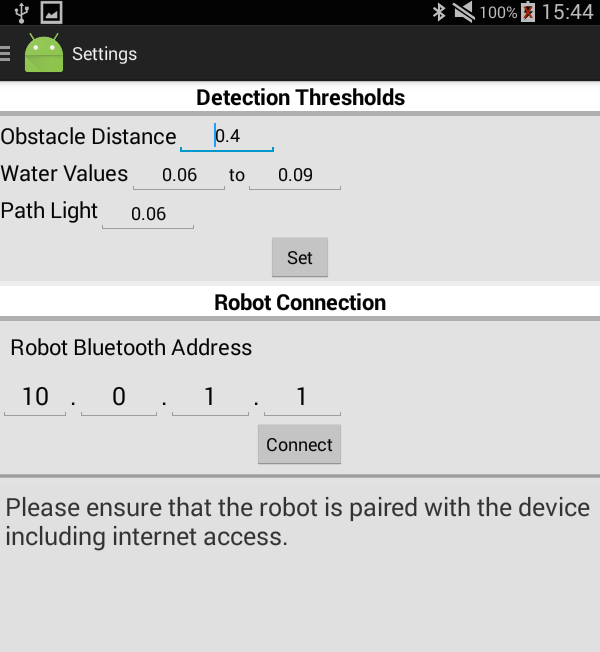
\includegraphics[scale=0.4]{settings.png}
\end{center}			
}
\par{This page is for connecting and disconnecting the application from the robot, you can also change the detection settings for the water, path and obstacle detection.}

\par{The detection settings at the top consist of:
\begin{description}
	\item[Obstacle Distance] This is the distance and which an obstacle is detected in front of the robot, the obstacle is detected between 0 and the value specified. The default is 0.4.
	\item[Water Values] This is the light values which detect when there is blue beneath the light sensor. The detection happens when the value fall between the values specified with the lower value on the left and the larger value on the right. The default values are 0.06 to 0.09.
	\item[Path Value] This is when the robot detects black beneath the light sensor indicating a path. The path is detected between the values of 0 to the value specified. The default is 0.06.
\end{description}
}
\clearpage
\par{The robot connection settings consist of:
\begin{description}
	\item[Robot Address]This is the address of the robot to be connected to, the value can be found on the robot when it is turned on. The default value is 10.0.1.1.\\
		\begin{center}
			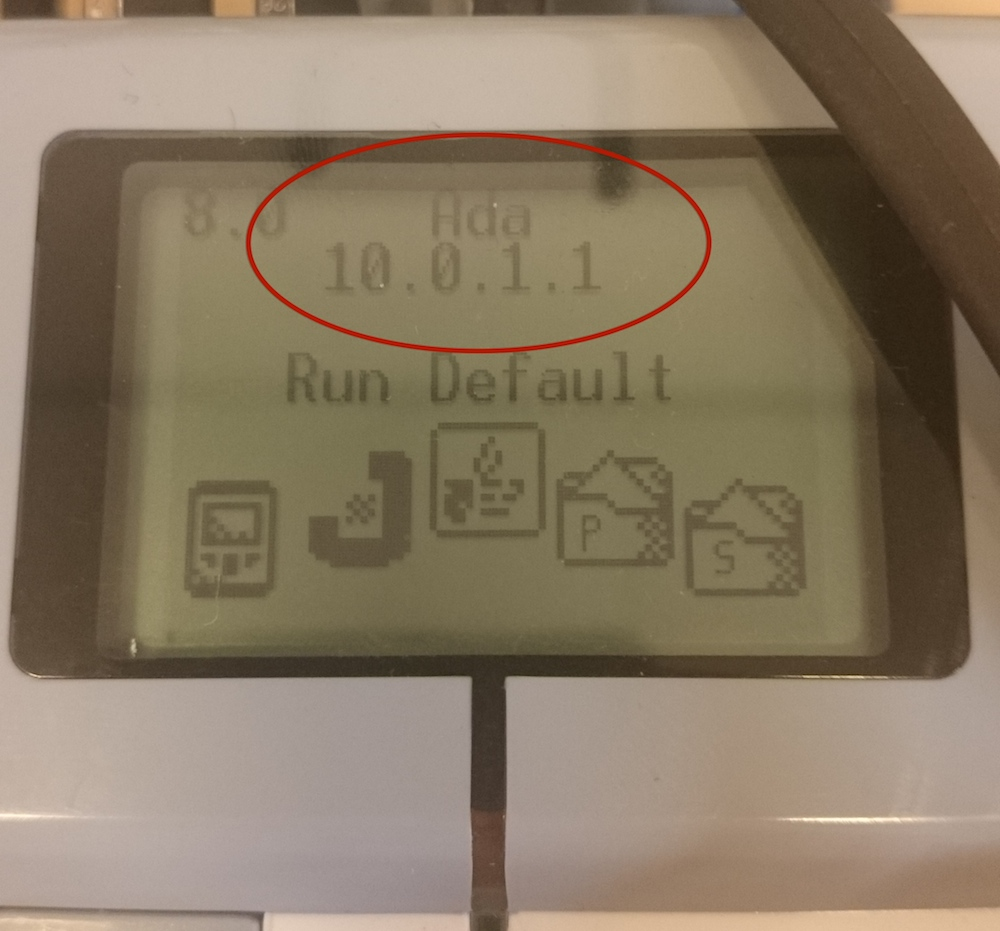
\includegraphics[scale=0.2]{address.JPG}
		\end{center}		
	\item[Connect/Disconnect] This button connects and disconnects the robot depending if there is a connection. The connection and disconnection process takes a few moments and when the process is happening it is described in the box below the button.
	\par{When using the app be sure to turn off WiFi and mobile data, as this does cause the app to be unable to connect to the robot.}
\end{description}
}
\end{document}  